
%%%%%%%%%%%%%%%%%%%%%%%%%%%%%%%%%%%%%%%%%
% Academic Title Page
% LaTeX Template
% Version 2.0 (17/7/17)
%
% This template was downloaded from:
% http://www.LaTeXTemplates.com
%
% Original author:
% WikiBooks (LaTeX - Title Creation) with modifications by:
% Vel (vel@latextemplates.com)
%
% License:
% CC BY-NC-SA 3.0 (http://creativecommons.org/licenses/by-nc-sa/3.0/)
% 
% Instructions for using this template:
% This title page is capable of being compiled as is. This is not useful for 
% including it in another document. To do this, you have two options: 
%
% 1) Copy/paste everything between \begin{document} and \end{document} 
% starting at \begin{titlepage} and paste this into another LaTeX file where you 
% want your title page.
% OR
% 2) Remove everything outside the \begin{titlepage} and \end{titlepage}, rename
% this file and move it to the same directory as the LaTeX file you wish to add it to. 
% Then add \input{./<new filename>.tex} to your LaTeX file where you want your
% title page.
%
%%%%%%%%%%%%%%%%%%%%%%%%%%%%%%%%%%%%%%%%%

%----------------------------------------------------------------------------------------
%	PACKAGES AND OTHER DOCUMENT CONFIGURATIONS
%----------------------------------------------------------------------------------------

\documentclass[11pt]{article}

\usepackage[utf8]{inputenc} % Required for inputting international characters
\usepackage[T1]{fontenc} % Output font encoding for international characters
\usepackage{graphicx}
\usepackage{grffile}
\usepackage{mathpazo} % Palatino font
\usepackage{indentfirst}
\usepackage[section]{placeins}
\usepackage{url}
\usepackage{hyperref}

\begin{document}



%----------------------------------------------------------------------------------------
%	TITLE PAGE
%----------------------------------------------------------------------------------------

\begin{titlepage} % Suppresses displaying the page number on the title page and the subsequent page counts as page 1
	\newcommand{\HRule}{\rule{\linewidth}{0.5mm}} % Defines a new command for horizontal lines, change thickness here
	
	\center % Centre everything on the page
	
	%------------------------------------------------
	%	Headings
	%------------------------------------------------
	
	\textsc{\LARGE Université Paris Dauphine}\\[1.5cm] % Main heading such as the name of your university/college
	
	\textsc{\Large Master 1 MIAGE}\\[0.5cm] % Major heading such as course name
	

	
	%------------------------------------------------
	%	Title
	%------------------------------------------------
	
	\HRule\\[0.4cm]
	
	{\huge\bfseries Projet d'Intelligence Artificielle}\\[0.4cm] % Title of your document
	
	\HRule\\[1.5cm]
	
	%------------------------------------------------
	%	Author(s)
	%------------------------------------------------
	
	\begin{minipage}{0.4\textwidth}
		\begin{flushleft}
			\large
			\textit{Réalisé par :}\\
			Lyes \textsc{MEGHARA}\\ % Your name
			Nadia \textsc{MSELLEK}\\ % Your name
		\end{flushleft}
	\end{minipage}
	~
	\begin{minipage}{0.4\textwidth}
		\begin{flushright}
			\large
			\textit{Encadré par :}\\
			Mr Stephane \textsc{AIRIAU}% Supervisor's name

		\end{flushright}
	\end{minipage}
	
	% If you don't want a supervisor, uncomment the two lines below and comment the code above
	%{\large\textit{Author}}\\
	%John \textsc{Smith} % Your name
	
	%------------------------------------------------
	%	Date
	%------------------------------------------------

	
	
	\vfill\vfill % Position the date 3/4 down the remaining page
	
	{\large18 Décembre 2017} % Date, change the \today to a set date if you want to be precise 

	
	%------------------------------------------------
	%	Logo
	%------------------------------------------------



	\leavevmode \newline 	\leavevmode \newline 	\leavevmode \newline 	\leavevmode \newline 	\leavevmode \newline 
	
\includegraphics[width=0.6\textwidth]{dauphine.png}\\[1cm] % Include a department/university logo - this will require the graphicx package


	 
	%----------------------------------------------------------------------------------------
	

	
\end{titlepage}

%----------------------------------------------------------------------------------------

\vspace{\stretch{3}}



\section{Introduction}


La notion de réseaux de neurones artificiels a été évoquée depuis plus de cinquante ans. Cela a permis l’évolution concrète de l’intelligence artificielle au plus grand bonheur des informaticiens et étudiants. Le projet que nous allons exposer traite de la capacité d’un algorithme d’apprentissage supervisé. \newline  \newline
Nous disposons pour cela d’une base de données créée par Yann \textsc{LECUN} nommée « \textit {Mnist handwritten database} » composée de plusieurs milliers d’exemples d’images de 28*28 pixels chacune représentant un chiffre manuscrit. \newline
Notre objectif est de récupérer parmi cette base de données un fichier input contenant 60 000 exemples sur lesquels notre algorithme va « apprendre » et ainsi pouvoir prédire les chiffres contenus sur chacun des 10 000 exemples donnés pour le test.\newline \newline 
Nos résultats sont exposés dans la section Résultats. 


\section{Outils de développement}

Dans le cadre de ce projet, nous avons utilisé GitHub pour une meilleure collaboration, eclipse sous la JDK 1.8, Doxygène nous a permis de générer une documentation visible depuis le fichier index.html. \newline Pour finir ce rapport a été rédigé en utilisant LateX.



\section{Résultats des tests}

Avec un SingleLayer, l'exécution pour 28*28 neurones d'entrées ainsi que 10 neurones de sorties dure 5 minutes, cette dernière corrige lentement le taux d'erreurs et avoisine les 8\%
 à la fin de l'exécution. \newline

Un HiddenLayer, cette fois-ci, avec 10 neurones cachés donne à priori les mêmes résultats pour le même temps d'exécutions, en revanche, en passant à 20 neurones cachés, les courbes se croisent, celle du réseau caché passe en dessous comme visible à la figure 2, augmenter le nombre des neurones cachés améliore l'apprentissage, mais ralentit fortement l'exécution.\newline

\begin{figure}[!htb]
  \centering
    \caption{Résultat d'entrainement d'un SingleLayer}
    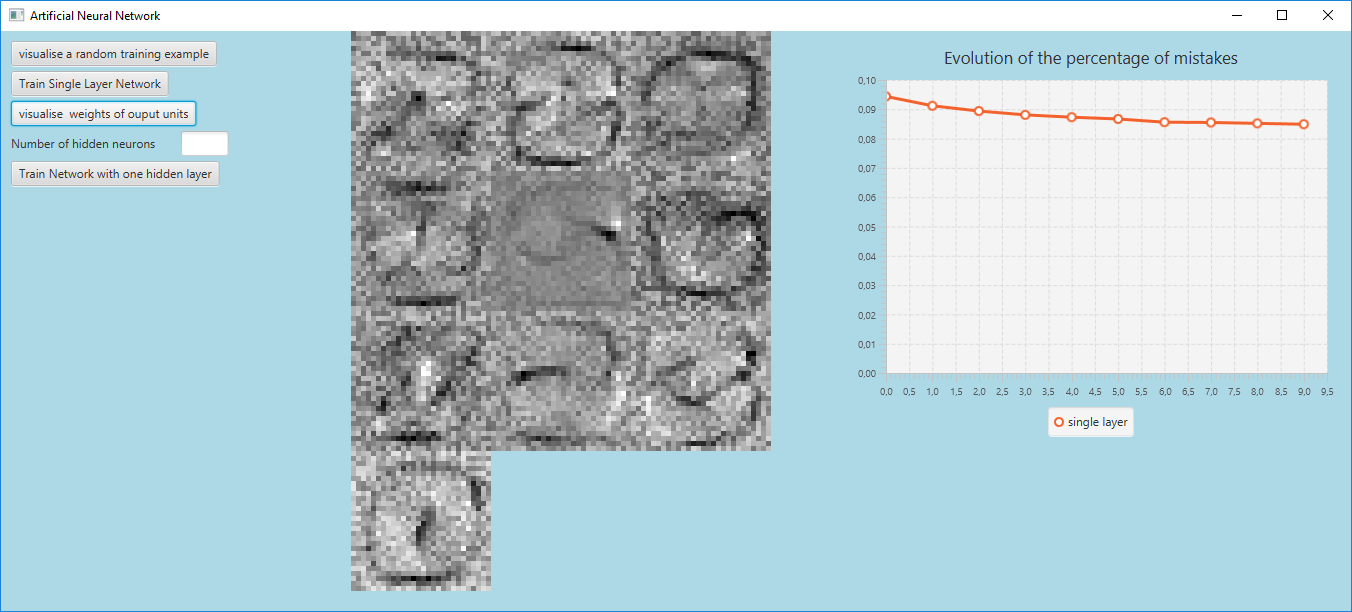
\includegraphics[width=\textwidth]{single.png}
	\textit {The training of your single layer lasted for 310.314633146 seconds}
\newline \newline

  \centering
    \caption{Résultat d'entrainement d'un HiddenLayer}
    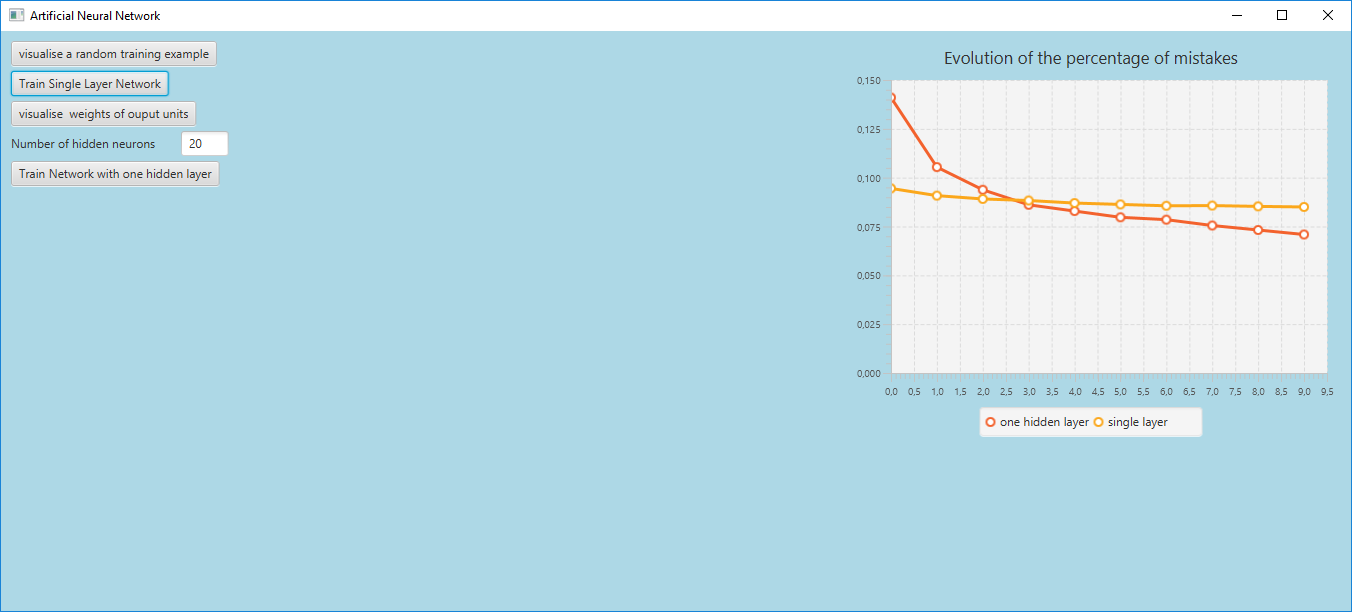
\includegraphics[width=\textwidth]{hidden.png}
	\textit {The training of your hidden layer lasted for 662.522861786 seconds}

\end{figure}




\section{Conclusion des résultats}

Blablablabla Blablablabla Blablablabla BlablablablaBlablablablaBlablablablaBlablablablaBlablablablaBlablablablaBlablablabla Blablablabla Blablablabla BlablablablaBlablablablaBlablablablaBlablablablaBlablablablaBlablablablaBlablablabla Blablablabla Blablablabla BlablablablaBlablablablaBlablablablaBlablablablaBlablablablaBlablablablaBlablablabla Blablablabla Blablablabla BlablablablaBlablablablaBlablablablaBlablablablaBlablablablaBlablablablaBlablablabla
\clearpage

\section{Ressenti de l'implémentation}

Il est important de souligner que mis à part le cours, avant de travailler sur ce projet nous n’avions pas d’expérience avec les réseaux de neurones artificiels. \newline
En outre, la première difficulté a été de comprendre le code déjà existant, les différentes classes et le lien entre ces dernières, comme les méthodes s'appellent et sont liées entre elles, trouver la source de nos erreurs n'a pas toujours été une tâche aisée.  \newline  \newline
Une des principales difficultés relevées a été l’implémentation des fonctions train pour les deux classes SingleLayer et OneHiddenLayer, qui chacune affichait une courbe constante avant correction de notre part. \newline
En revanche, les fonctions feed ont été assez simples à implémenter étant fluide de sens et de logique.

\section{Améliorations éventuelles / Hypothèses }

Le programme étant assez lent à tourner, une des premières idées que nous avons eues, était d'accroitre sa vitesse, en passant par des Threads, solution qui n'a pas été implémentée par manque de temps. \newline \newline
D'autres points, sur le côté théorique cette fois-ci, l'utilisation de biais n'a pas été mentionnée de façon explicite dans ce cours.  \newline
Par ailleurs, l'algorithme d'apprentissage \textit {Widrow-Hoff} a été préféré à \textit {l'algorithme de gradient}, étant à la fois plus efficace, et plus simple à implémenter.

\clearpage

\section{Webographie} 
\begin{itemize}
\item \url{https://fr.wikipedia.org/wiki/Perceptron} \newline
\item \url{https://fr.wikipedia.org/wiki/Perceptron_multicouche} \newline
\item \url{alp.developpez.com/tutoriels/intelligence-artificielle/reseaux-de-neurones/} \newline
\item \url{https://youtu.be/L7WNYvbvGBc} \newline
\item \url{https://github.com/mattm/simple-neural-network/blob/master/neural-network.py} \newline
\item \url{https://github.com/nathansegan/mnist_neural_network/blob/master/src/neural_net.py} \newline
\item \url{https://www.cs.cmu.edu/afs/cs/academic/class/15883-f15/slides/backprop.pdf} \newline
\item \url{http://www.dgp.toronto.edu/people/RMB/papers_old/p6.pdf} \newline
\item \url{https://www.labri.fr/perso/nrougier/downloads/Perceptron.pdf} \newline

\end{itemize}

\end{document}
